\documentclass[../main.tex]{subfiles}

\begin{document}
\subsection{Business products}
        Technology and \textsc{ai} advancements have been changing human lives for the better.
	The possible opportunities for innovation and creativity are unlimited. This
	project has many aspects that could lead to business opportunities and commercial
	prototypes. 
	One of the many commercial products that could come out of this project is
	the \gls{drl} object detection model. This model can be used in any system
	that requires object detection. It could be a \gls{uav}, a \textsc{cctv} camera, or
	any system that inputs an image to the model after being trained on a similar 
	dataset.
	Depending on the system, the \gls{drl} model could be trained using a different
	dataset to detect a different object (e.g. cars, humans, animals).
	Another possible product is the \gls{drl} model responsible for navigating the
	drone after being trained on a specific movement pattern.
	Moreover, the entire system developed in this project is a viable product.
	
\subsection{Drone market growth}
	According to \textcite{Atwater15Commercial}, the global market of drones is 
	increasingly becoming a key player in both military and civilian applications. 
        The number of \uavs in use in 2040 is expected to 
        be \SI{1.2}{million} \cite{Amo19}. In addition,
	the net value of the \glspl{uav} industry is estimated to reach 13 billion dollars
	by 2024 as illustrated in~\cref{fig:drone-market}%
        ~\cite{Mic14}. This is due to the efficiency 
	and flexibility of \glspl{uav} in completing various tasks. 
	Moreover, \textcite{Yes19} states that there will be a steady annual growth of 
	15-20\% during the next decade, and major companies like Google and Tesla are investing
	in the \gls{uav} industry. Their research also forecasts that integrating drones in
	different sectors will have an economic impact of 82 billion dollars between 2015 
        and 2025 \cite{Yes19}.
	
\begin{figure}[tbp] 
        \centering
        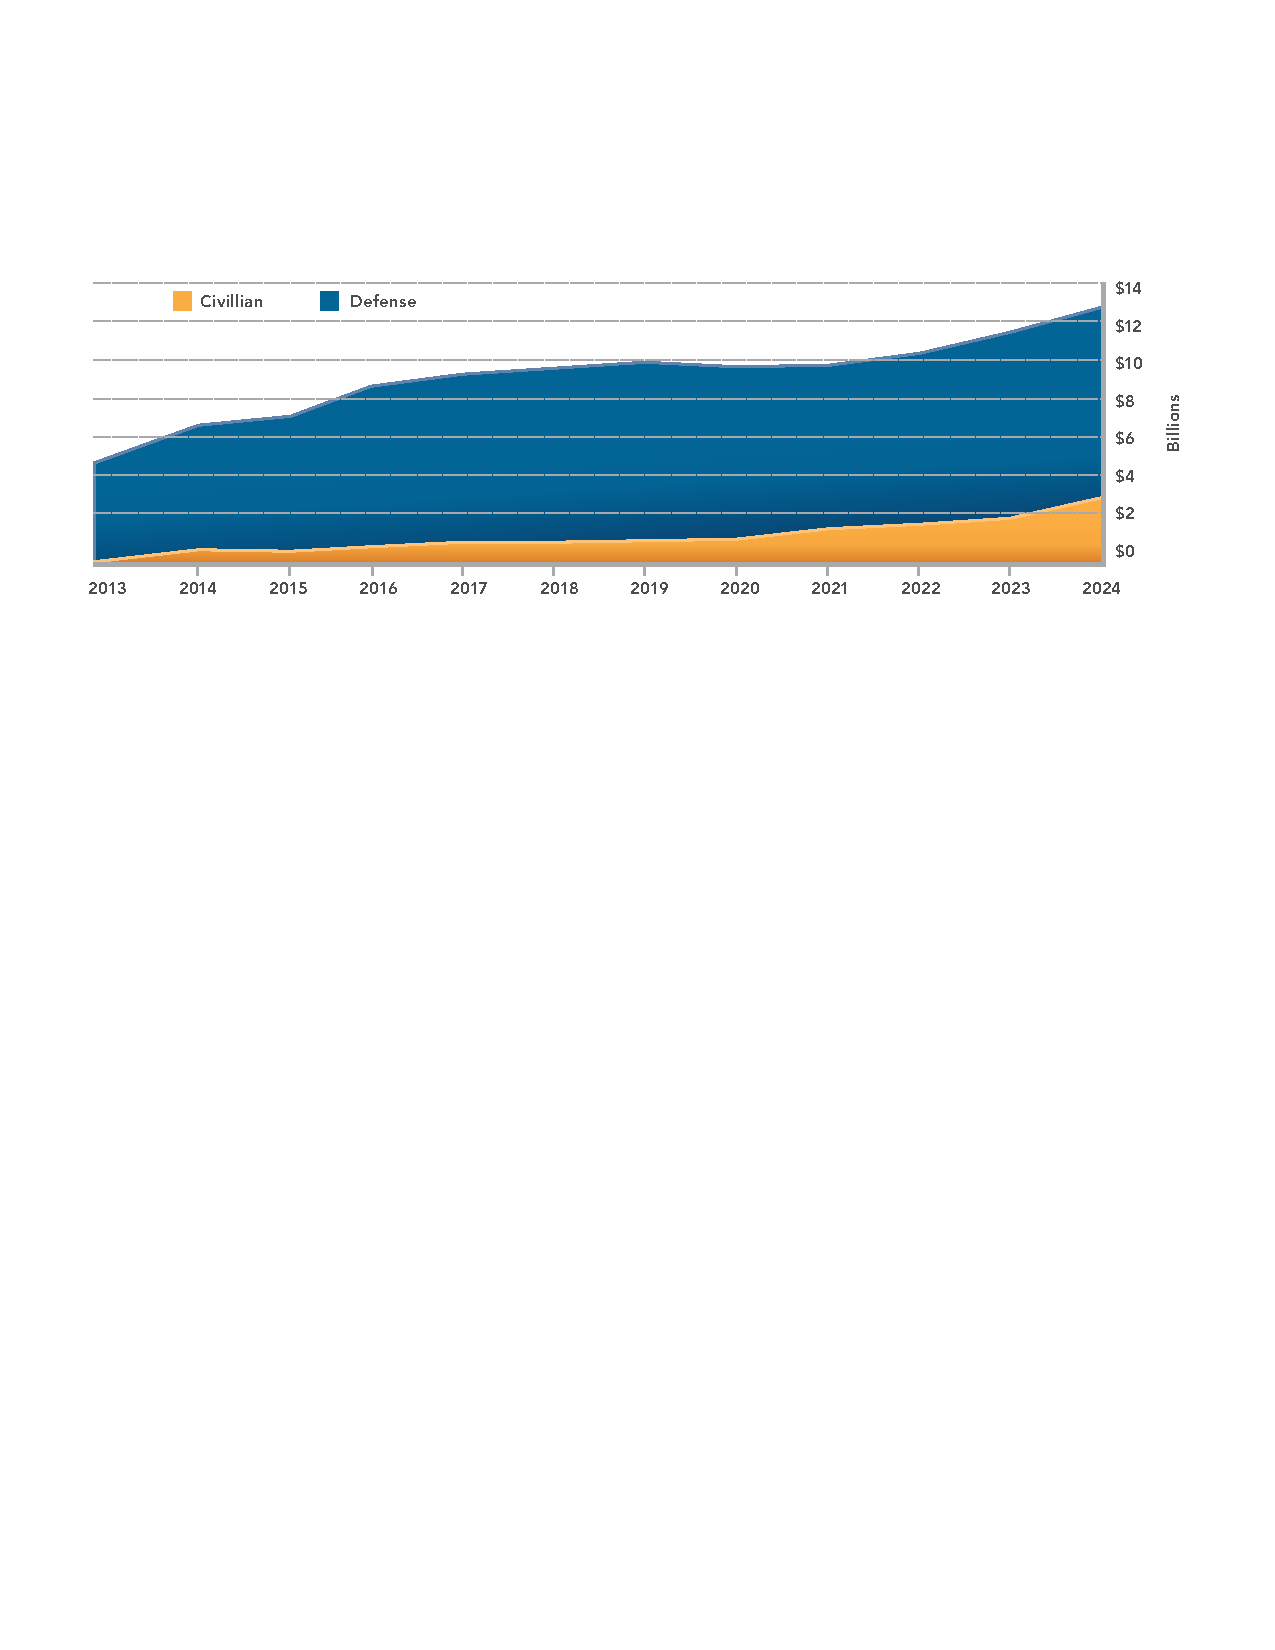
\includegraphics[width=1.0\textwidth]{drone-market}
        \caption[The forecasted global drone market.]
        {The forecasted global drone market~%
        \cite[Fig.~2]{Mic14}.} 
        \label{fig:drone-market} 
\end{figure}
	
\subsection{Interested parties}
	Many companies and stakeholders would be interested in acquiring either the
	complete system that we produce, or sub-parts (e.g. \gls{drl} model). Some of them include:
	\begin{enumerate}
		\item Military bodies -- drones and object detection models could 
		be used in military operations to detect people of danger, secure 
		sensitive areas, and even eliminate threats (i.e. drone weaponry).
		
		\item Biological research institutes -- 
                    the \gls{uav} along with the object
		detection model that we provide could be trained to detect certain animals 
		and track them. This would revolutionize biological research.
		
		\item Security companies -- personal home security could be established through
		\glspl{uav} and such object detection models could detect threats or unusual
		behaviors. This is applicable in any public area or even personal properties.		
		
	\end{enumerate}

\subsection{Viability in Qatar}
	Our product is simple enough to be used by anyone. However, it is mostly intended for 
	authorized institutes that have a license to fly \glspl{uav} as the legal limitations 
	in the region are very strict. 
	Many of the possible applications are for out of town use (e.g. biological research), 
	and this makes the product more acceptable to the public as it does not invade anyone's privacy.
	Moreover, one of the major advantages of our product is that there is no competitor 
	inside Qatar as most drones in Qatar are used for photography purposes, and our
	specific product idea has never been deployed in the country. Therefore, this gives us an excellent 
	market head start and implies the huge market need for such a product.

\subsection{Product Price}

To choose an acceptable price, we must analyze the different components of the system. Their prices are listed in the \cref{tab:components-prices}.

\begin{table}[H]
\begin{center}
        \caption{A price list of the system components.}
        \label{tab:components-prices}
        \begin{tabular}{p{3.5cm} c c} 
            \toprule
            \textbf{Component} & \textbf{Price(\$)} & \textbf{Price(\textsc{qr})}\\
                \midrule
                \anafi Drone & 800.00 & 2920.00 \\
                Raspberry Pi & 150.00 & 547.50 \\
                Raspberry Pi battery & 30.00 & 109.50\\
                Wi-Fi Dongle & 20.00 & 73.00\\
                \hline 
                Total & 1000.00 & 3650.00 \\
                Selling price & 1644.00 & 6000 \\ 
                Profit/unit & 644.00 & 2350 \\
                \bottomrule
        \end{tabular}
\end{center}
\end{table}

	The discussed prices might not be acceptable by individuals, but the product is mainly designed for big organizations who certainly can afford it.
	



\end{document}
